\documentclass[
	english,
	fontsize=10pt,
	parskip=half,
	titlepage=true,
	DIV=12
]{scrartcl}

\usepackage[utf8]{inputenc}
\usepackage{babel}
\usepackage[T1]	{fontenc}
\usepackage{lmodern}
\usepackage{microtype}
\usepackage{color}
\usepackage{csquotes}
\usepackage{xspace}

\usepackage{hyperref}

\newcommand*{\tabcrlf}{\\ \hline}

\usepackage{amsmath}
\usepackage{amssymb}
\usepackage{dsfont}
\usepackage[arrowdel]{physics}
\usepackage{mathtools}
\usepackage{siunitx}

\usepackage{minted}
	\usemintedstyle{friendly}

\newcommand*{\inPy}[1]{\mintinline{python3}{#1}}
\newcommand*{\ie}{i.\,e.\xspace}
\newcommand*{\eg}{e.\,g.\xspace}

\begin{document}

\part*{Python Problems 05, Summer 2021}
In this exercise, we will write code that reads text data files from the hard disk, displays them as a plot on screen and allows to superimpose one or more fits onto that data.

Some mathematical background is probably necessary to understand the finer details of this sheet. If you feel like you don't know what a Fourier spectrum is, leave out this part and focus on the curve fit part.

While you have seen the elementary ideas on how to use tkInter in class, many details were not covered. This is by design: looking up things online is an essentail part of the day-to-day business of any programmer. I've put some links in the description below, but you might find it useful to use your search engine of choice every once in a while. In general, it is a good idea to search for terms matching the pattern \texttt{tkinter verb details}, \eg \texttt{tkinter set font color}. Usually, searching for English terms yields more and better results than trying to find resources in other languages.

Likewise, this problem statement offers a guideline in which order to attack the individual subproblems, but lets you find \emph{your} solution on your own. I'm sure in the long run, you'll appreciate the chance to find your own structure, even if this might lead you into dead ends every so often.

The features to implement are rather extensive, but just see how far you get, and feel free to omit parts of this sheet. For example, you can leave out the Fourier analysis/synthesis part of this problem statement or drop the fit part alltogether.

Note that this could have been a valid final project code. Also note that my solution has exactly 666 lines of code ;)

\section{Load File Dialog}
Familiarize yourself with the open file dialog as provided by the tkInter module. Read up on \url{https://tkdocs.com/tutorial/windows.html#dialogs}, then test what you've just found by writing a short code that allows the user to select a file from their hard disk. Print the selected filename on the console.

You can make it such that the dialog only shows files with certain extensions. For that, an optional argument \texttt{filetypes} can be passed to the function \texttt{askopenfilename}. This optional argument should hold a \inPy{list} of \inPy{tuple}s of \inPy{str}ings. Each \inPy{tuple} comprises of two strings, the first of them being a description for the user and the second one describing the file pattern. A file pattern is a string comprising \emph{wildcard} the character \texttt{*} (think of it as a joker) and any mandatory characters that should be filtered for. Example: \inPy{"*.py"} would be the file pattern that matches all files with the extension \texttt{py}.

Use this knowledge to adjust your code such that the resulting dialog allows the user to select CSV files (\texttt{*.csv}), Text files (\texttt{*.txt}) or Any files (\texttt{*}). The resulting dialog should look like this:
\begin{center}
	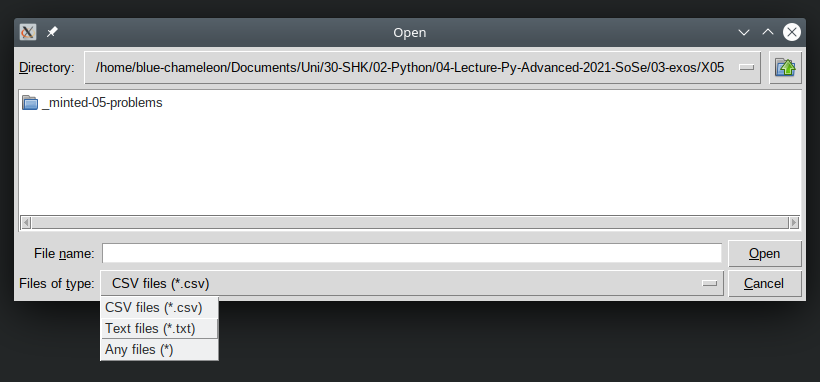
\includegraphics[width=.6\linewidth]{./tk-filepicker}
\end{center}

\section{Matplotlib in tkInter}
The search term \texttt{matplotlib in tkinter frame} leads to this ressource: \url{https://matplotlib.org/3.1.0/gallery/user_interfaces/embedding_in_tk_sgskip.html}
Read and understand the example shown there. Focus on the \texttt{canvas}, and forget about the \texttt{NavigationToolbar2Tk} and the \texttt{key\_press\_handler}.

Then generate a TK window with a button and a dummy MatPlotLib plot.

\section{Widgets Layout}
Now, generate the main window as shown below. For the time being, forget about what functions the buttons serve, but only try to write code that produces an user interface that looks as close as possible to the one shown on this problem sheet:
\begin{center}
	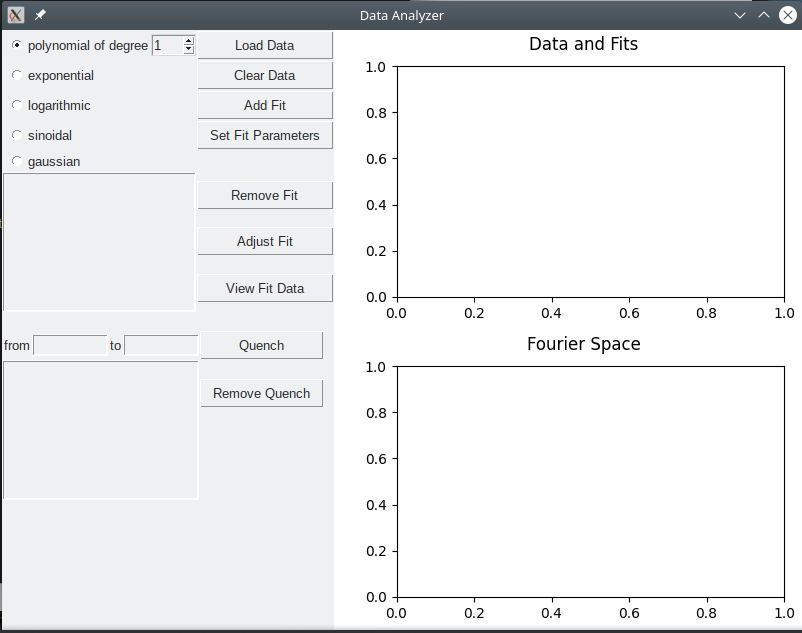
\includegraphics[width=.8\linewidth]{./tk-MainWin}
\end{center}
Note that the big boxes are Listboxes and the small boxes next to the labels "from" and "to" are Entries. The widget next to the Radiobutton "polynomial of degree" is a Spinbox.

Begin by analyzing the structure of the arrangement: What can be put in frames, grids, ...? Then populate your window with the various widgets, but leave them defunct for the time being. However, do keep in mind which controls need to be read later on or need to be linked to some tk variable. Store handles to those widgets or variables where necessary.

\section{Aim}
In this section we clarify what we want to do. No code to be written ;)

By clicking on the \emph{Load Data} button, the user should be prompted a dialog that asks them to specify a file to be loaded, much as we've seen how to do in the first task. The load dialog should filter for CSV files, but also have the option to filter for TXT files or apply no filter at all.

The button \emph{Clear Data} should make it such that the Program falls back into its pristine state, \ie all data are to be expunged from memory and the display should be as if the program was just started.

Clicking \emph{Add Fit} should compute a fit to the loaded data. The type of fit can be selected by use of the Radiobuttons and the Spinbox. As you remember, SciPy's \texttt{curve\_fit} function often fails if no initial guess is provided. To that end, clicking on \emph{Set Fit Parameters} should allow the user to provide this initial guess in a separate dialog window.\\
It should be possible to add multiple fits to the same basic data. All fits are to be listed in the Listbox just below the Radiobutton \emph{gaussian}.

Unsuccessful fits can be removed by selecting the relevant attempt from the Listbox and clicking \emph{Remove Fit}.

\emph{Adjust Fit} should allow the user to alter the label and color associated with a fit. Clicking \emph{View Fit Data} should display the fit parameters as well as the Covariance Matrix (both are returned by SciPy's \texttt{curve\_fit}).

The loaded data as well as the fitted graphs should then be shown in the \emph{Data and Fits} plot; its Fourier Transform (as computed by SciPy's FFT) are to be rendered in the \emph{Fourier Space} part.

Measured data are often noisy, as can be seen in the screenshot below. Often, noise can easily be reduced by setting some components in the Fourier spectrum to zero. The text boxes next to \emph{from} and \emph{to} specify the entries that are to be set to 0, when the button \emph{Quench} is clicked. The listbox below lists all the suppressed modes. Selecting one and clicking \emph{Remove Quench} should undo the action. It should be possible to suppress several parts of the Fourier spectrum independently from one another.

The fit features should use the noise-reduced data (\ie the result of SciPy's inverse Fourier Transform) for the fit, if any modes have been quenched.

The program in use could look like this:
\begin{center}
	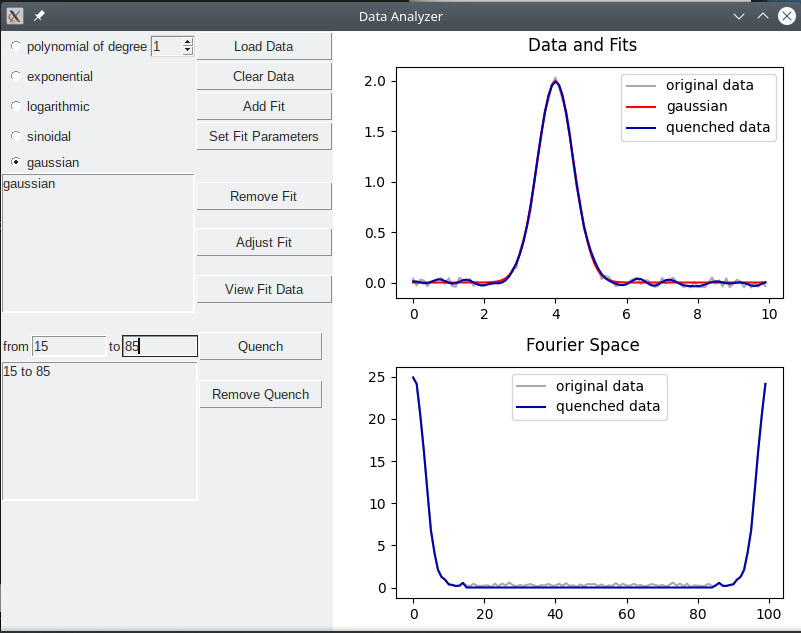
\includegraphics[width=.6\linewidth]{./tk-MainWin-used}
	\qquad
	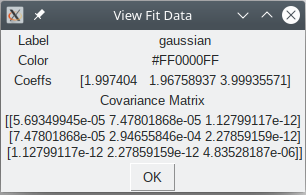
\includegraphics[width=.25\linewidth]{./tk-ViewFitData}
\end{center}

You will find several CSV files on GRIPS that you can use to test your code with. You will also find the code \texttt{generateData.py} that was used to create these CSV files.

\section{Showing and Clearing Plots}
Think now of how to represent the plot data in memory and where to instantiate them (\ie in which scope). You will need X- and Y-Data for the original data, as well as Frequency- and Intensity-Data for the Fourier spectrum. In this case, it is convenient to work with global variables.

First make it so that some default plot is rendered, simply for testing. Now implement the functionality of the button "Clear Data", such that erases all data in memory and resets the plot areas. Once this works, implement the functionality of the \emph{Load Data} button. Leave the Fourier spectrum out for the time being.

\emph{Hint:} The method \texttt{axesobject.cla()} restores a pristine drawing area.

\emph{Hint:} If you followed the example from task 2, the MatPlotLib figure has been \enquote{captured} by the TK system. Changes are not automatically rendered on screen. Instead, you'll need a call to \texttt{canvas.draw()} each time you want to make changes visible.

\emph{Hint:} You can add/change the function of a Button \emph{after} it has been created. To do so, use \texttt{handleToButton["command"] = function}.

\emph{Hint:} If you're using global variables, you can only alter them in your functions if you declared them \inPy{global} there. Read up on the declaration in the Python script (Chapter 6.3).

\section{Fourier Space}
Now extend your code so that loading a file first resets the application memory. After the real space data are loaded, the Fourier transform should automatically be computed and displayed.

Once this works, attack the Quench-Feature. Clicking the \emph{Quench}-Button should create a copy of the Fourier spectrum and set the range indicated by the text boxes \emph{from} and \emph{to} to zero. Each quenched part of the Fourier spectrum should be logged in the listbox. Selecting a line in the list box and pressing \emph{Remove Quench} should undo the selected action.

Make it so that each Quench/Undo-Action in the Fourier spectrum also affects the real space data: Once a copy of the Fourier spectrum is created, its inverse transform (as computed by SciPy's ifft) should be shown in the \emph{Data and Fits} section.

Also think of what happens when the user enters nonsensical values: display a messagebox instead of doing a Quench-Action then.

\section{Fits}
Now go about the curve fitting features. 

\subsection{Fit Prototypes}
We want the fit types to mean the following:
\begin{itemize}
\item polynomial of degree $N$: $\sum_{k=0}^N a_k x^k$
\item exponential: $a \exp( b(x - c)) + d$
\item logarithmic: $a \log( b(x - c)) + d$
\item sinoidal   : $a \sin( b(x - c)) + d$
\item gaussian   : $a \exp(-b(x - c)^2) + d$
\end{itemize}

First, make sure you have code that implements these functions.

\emph{Hint:} Variadic arguments are very useful for the polynomial function.

\emph{Hint:} Numpy's module \texttt{polynomial} implements a class \texttt{Polynomial} that can be used to evaluate a polynomial (duh).

\subsection{Initial Guess}
As you remember, SciPy's \texttt{curve\_fit} sometimes fails if no initial guess is given. To that end, we need a new dialog where the user can provide this initial guess. This dialog should offer a variable number of text boxes, depending on which kind of fit is currently selected. This dialog is to be shown when the user clicks \emph{Set Fit Parameters} and could look like this:
\begin{center}
	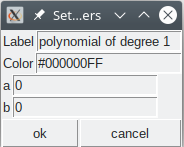
\includegraphics[width=.25\linewidth]{./tk-SetParams-a}
	\quad
	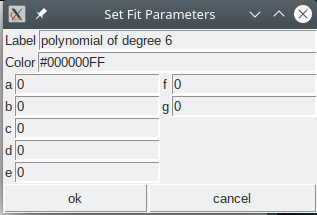
\includegraphics[width=.40\linewidth]{./tk-SetParams-b}
\end{center}

The user input then could be stored in a global variable \texttt{settings} that will later be used by the code running the \emph{Add Fit} button. Remember that, if you use this solution, you'll need to declare your \texttt{settings} variable \inPy{global}. Also, make sure that this \texttt{settings} variable holds reasonable values, even if \emph{Set Fit Parameters} has never been clicked at.

\emph{Hint:} A new dialog can be created by using \texttt{tk.Toplevel}.

\emph{Hint:} You may want to add a callback procedure (the \texttt{command=} feature) to your Radiobuttons and the Spinbox. This callback could set your \texttt{settings} to a well-defined default

We usually want our dialogs to be \emph{modal}, \ie while the dialog is active, the main window should not be accessible. (Imagine the dialog being active and someone clicks the button \emph{Set Fit Parameters} a second time). To that end, you can use the \texttt{grab\_set} method of your Toplevel window. That is, if you created your dialog window with the handle \texttt{dlg}, then \inPy{dlg.grab_set()} will prohibit any user interaction with other windows belonging to your code. This locked mode persists as long as either the modal dialog is destroyed (by closing the window or invoking \texttt{dlg.destroy()}), or until it is released with \inPy{dlg.grab_release()}.

\subsection{Add Fit}
Now, implement the \emph{Add Fit} button. It should take the initial guess provided by the global \texttt{settings} variable and feed it into SciPy's \texttt{curve\_fit}. Store the output of this function (the fit parameters as well as the covariance matrix) in a new global list, along with the label and the color of the fit in the plot. Compute the fit function values, too, and put them in your list as well. Make sure you're using the data reconstructed from the quenched Fourier spectrum, if they exist. Finally, plot the fitted function on screen. Add an element to the listbox in the \emph{Data and Fits} section, representing the newly added fit. Finally, think of the possibility of a failed fit. In this case, the code should abort and display a messagebox instead.

\emph{Hint:} the covariance matrix that \texttt{curve\_fit} returns is a 2D numpy array. If a fit fails, all elements of the matrix are \texttt{np.inf}.

\subsection{View Fit Data}
Of course we want not only to see the fitted function, but also know its details. To that end, make it such that clicking on \emph{View Fit Data} shows the following \emph{modal} dialog, if a line in the listbox indicating a fit was selected:
\begin{center}
	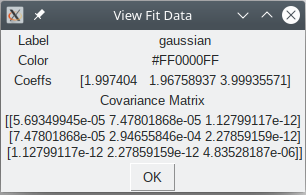
\includegraphics[width=.4\linewidth]{./tk-ViewFitData}
\end{center}

Other than the \emph{OK} button, there are only Labels in the window. The text next to \emph{Coeffs} is the String representation of the first return value of \texttt{curve\_fit}, \ie a NumPy array with the coefficients of the fit. Likewise, the text under \emph{Covariance Matrix} is the string rendition of the second return value of \texttt{curve\_fit}.

\subsection{Adjust Fit and Remove Fit}
There's only two more buttons to add functionality to!

\emph{Adjust Fit} should allow the user to rename a fit from the Listbox and change the color it is plotted in.\\
\emph{Remove Fit} should remove a fitted curve from memory and the plots.

Do so, and you have finished building a very useful tool for analyzing arbitrary data!
\end{document}
